\begin{figure}[h]
\centering
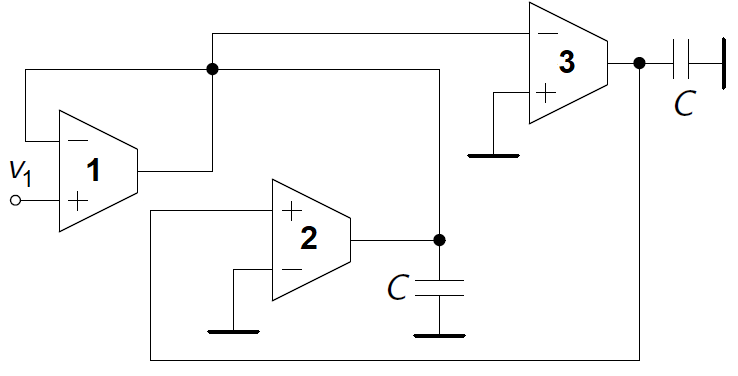
\includegraphics[scale=0.5]{v1.png}
\caption{Schéma zapojení OTA \label{s:V1}}
\end{figure}
\begin{figure}[h]
\centering
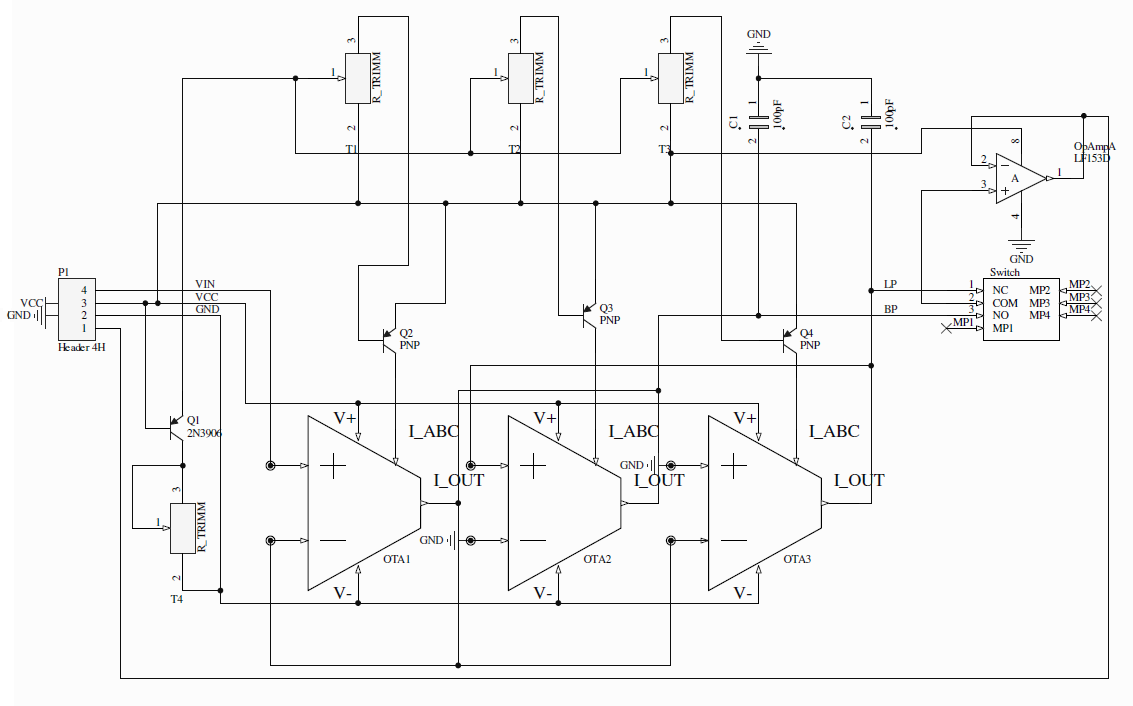
\includegraphics[scale=0.45]{schemev1.png}
\caption{Schéma s obvodovými prvky s řízeným napájením}
\end{figure}
\begin{figure}[h]
\centering
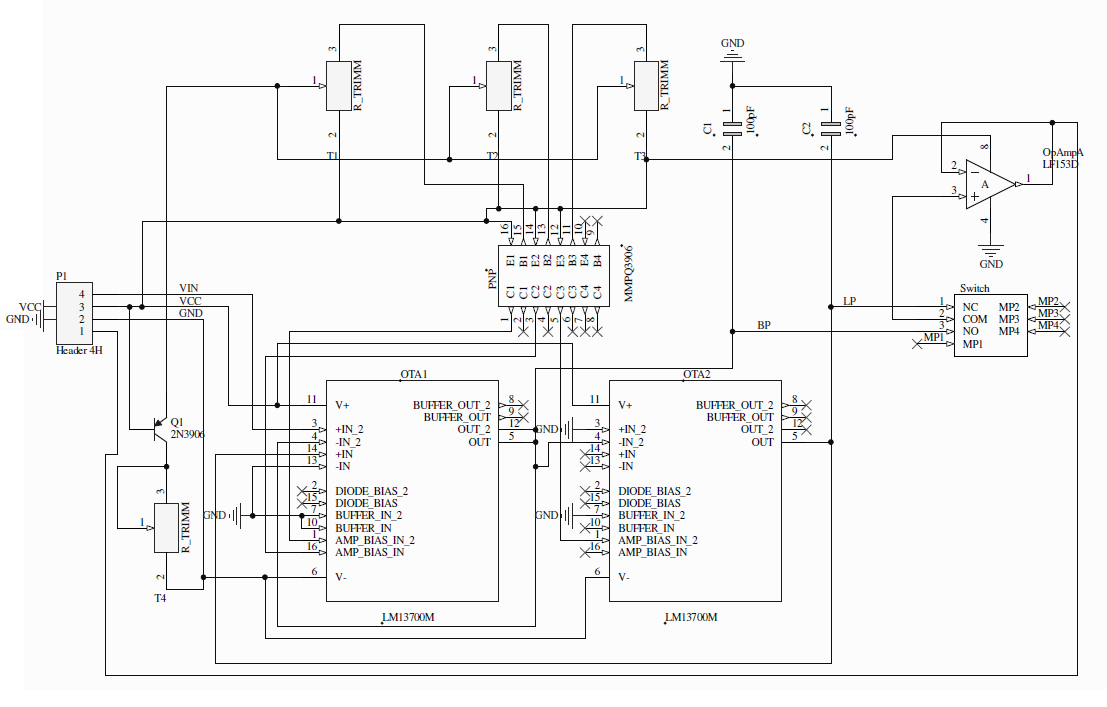
\includegraphics[scale=0.45]{v1schematics.png}
\caption{Schéma se zapojením IO s řízeným napájením}
\end{figure}
\begin{figure}[h]
\centering
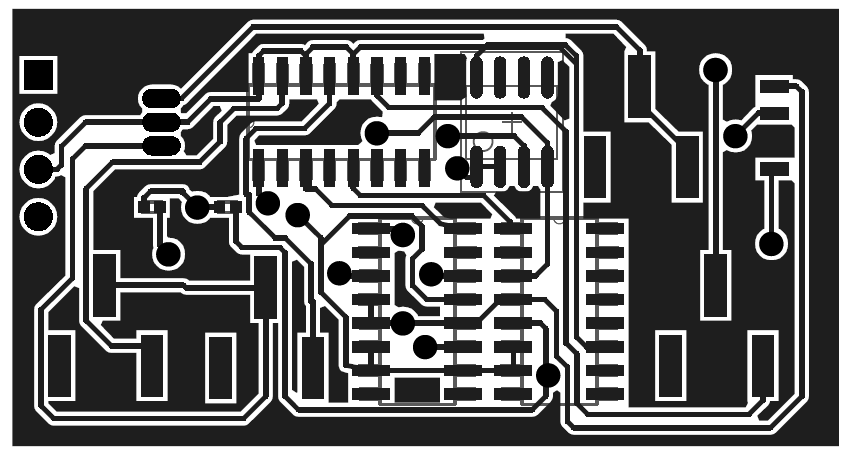
\includegraphics[scale=0.5]{v1top.png}
\caption{Horní strana DPS}
\end{figure}
\begin{figure}[h]
\centering
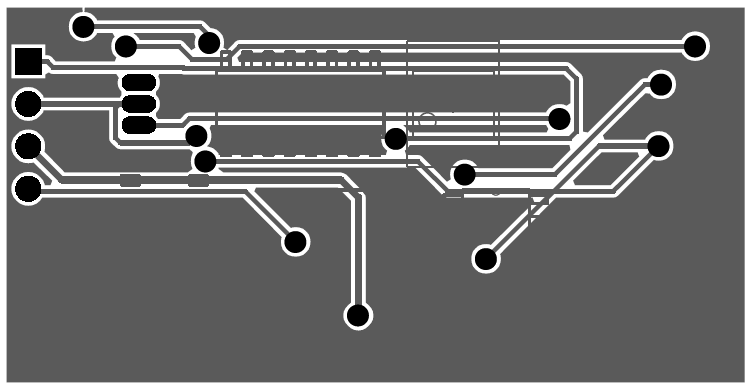
\includegraphics[scale=0.5]{v1bot.png}
\caption{Spodní strana DPS}
\end{figure}
\begin{figure}[h]
\centering
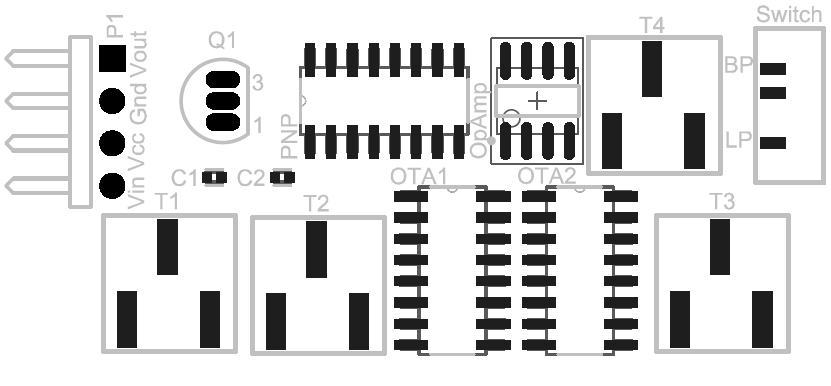
\includegraphics[scale=0.5]{v1assembly.png}
\caption{Rozmístění součástek}
\end{figure}
\begin{figure}[h]
\centering
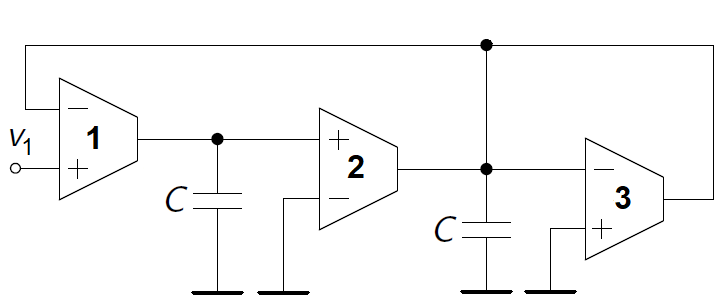
\includegraphics[scale=0.5]{v2.png}
\caption{Schéma zapojení OTA}
\end{figure}
\begin{figure}[h]
\centering
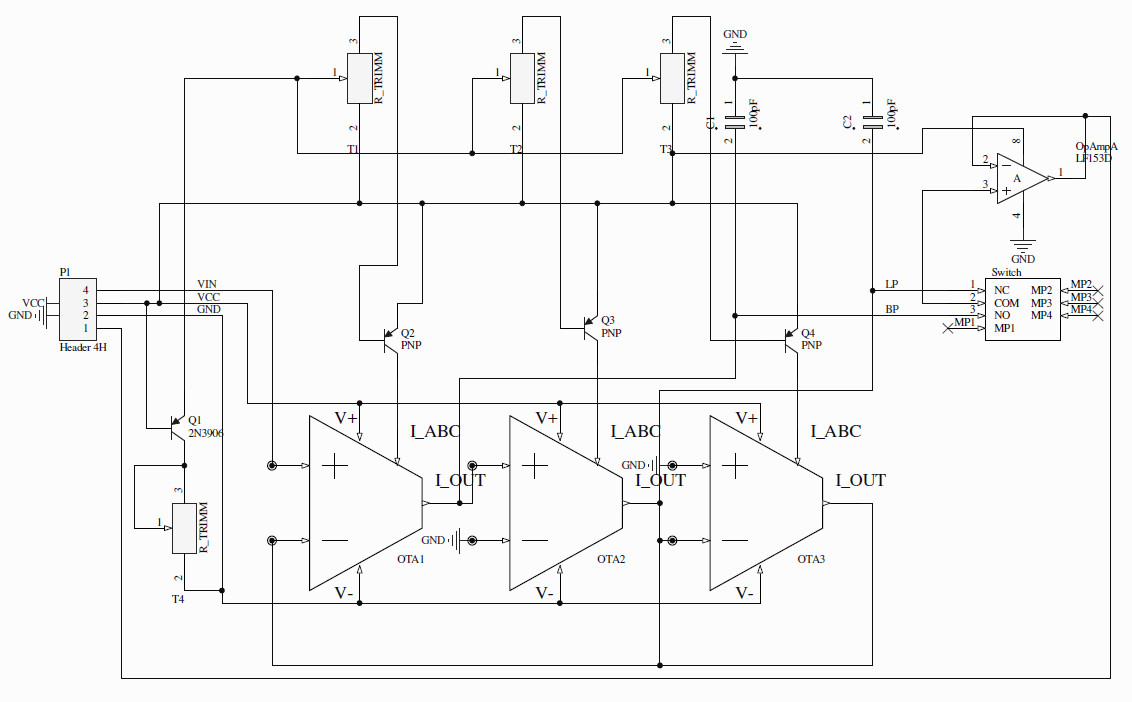
\includegraphics[scale=0.45]{schemev2.png}
\caption{Schéma s obvodovými prvky s řízeným napájením}
\end{figure}
\begin{figure}[h]
\centering
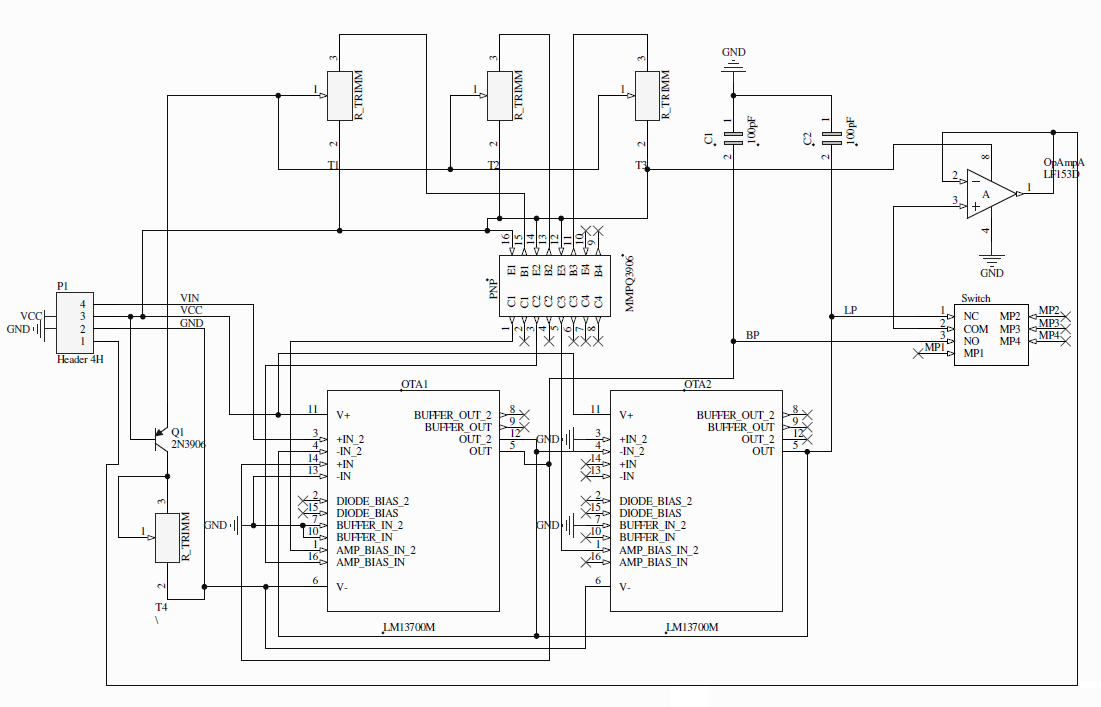
\includegraphics[scale=0.45]{v2schematics.png}
\caption{Schéma se zapojením IO s řízeným napájením}
\end{figure}
\begin{figure}[h]
\centering
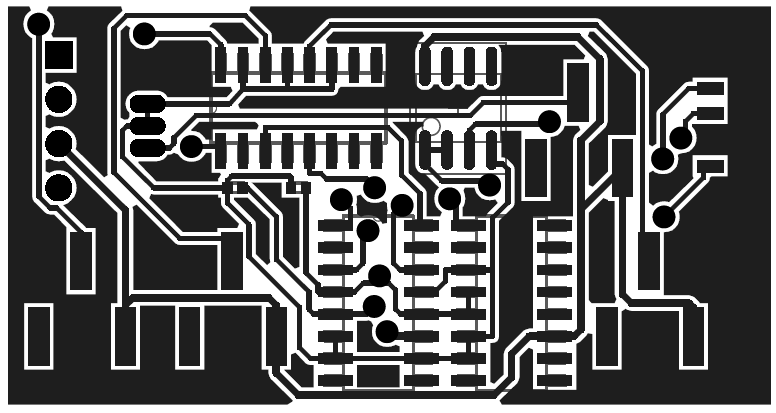
\includegraphics[scale=0.5]{v2top.png}
\caption{Horní strana DPS}
\end{figure}
\begin{figure}[h]
\centering
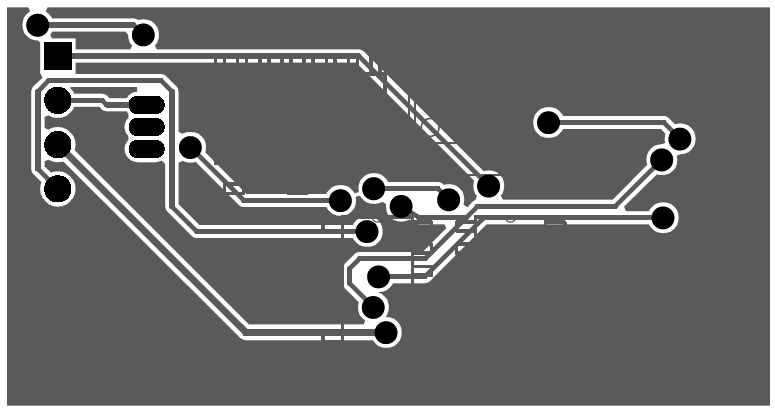
\includegraphics[scale=0.5]{v2bot.png}
\caption{Spodní strana DPS}
\end{figure}
\begin{figure}[h]
\centering
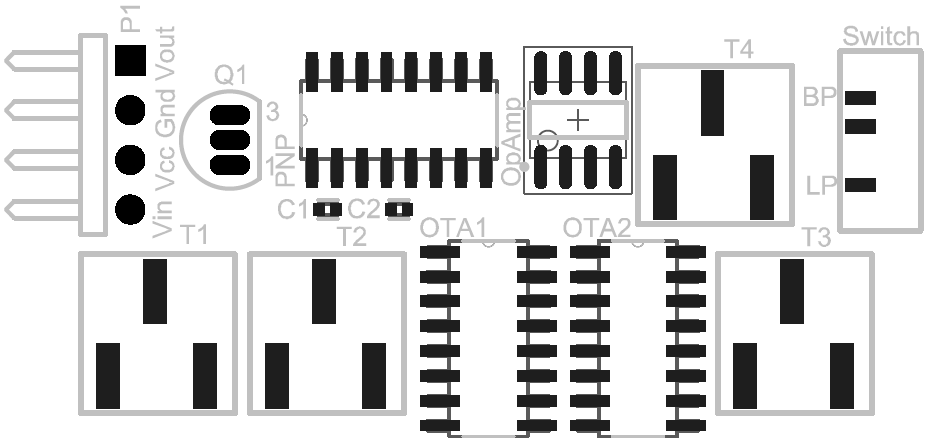
\includegraphics[scale=0.5]{v2assembly.png}
\caption{Rozmístění součástek}
\end{figure}
\begin{figure}[h]
\centering
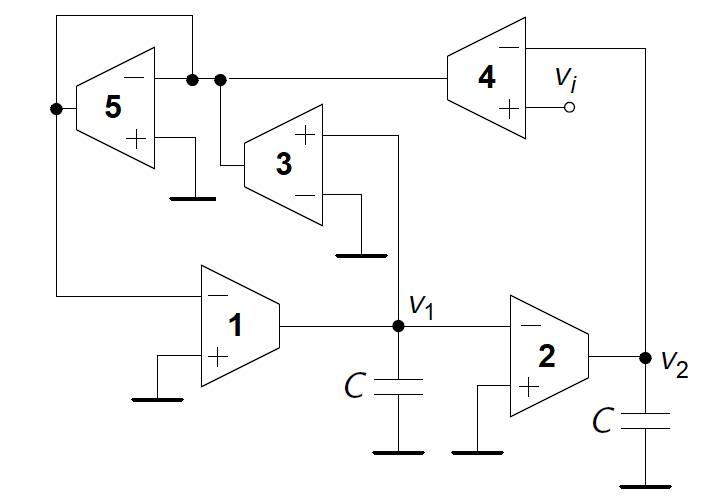
\includegraphics[scale=0.5]{v3.png}
\caption{Schéma zapojení OTA}
\end{figure}
\begin{figure}[h]
\centering
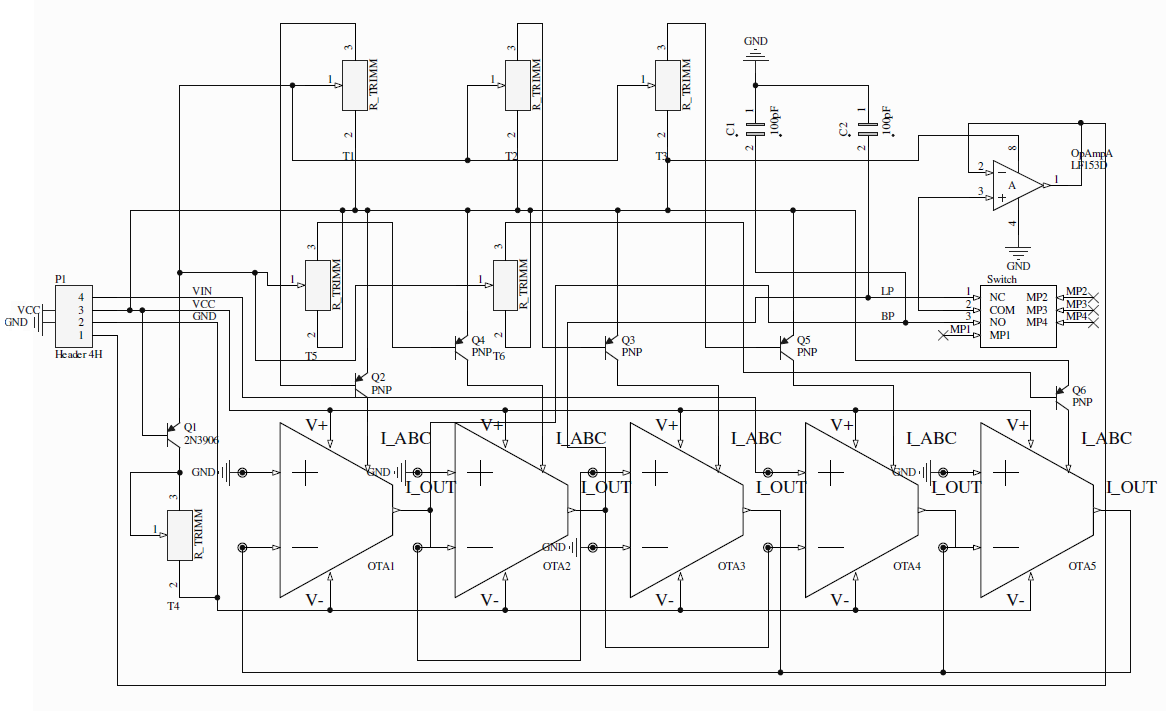
\includegraphics[scale=0.45]{schemev3.png}
\caption{Schéma s obvodovými prvky s řízeným napájením}
\end{figure}
\begin{figure}[h]
\centering
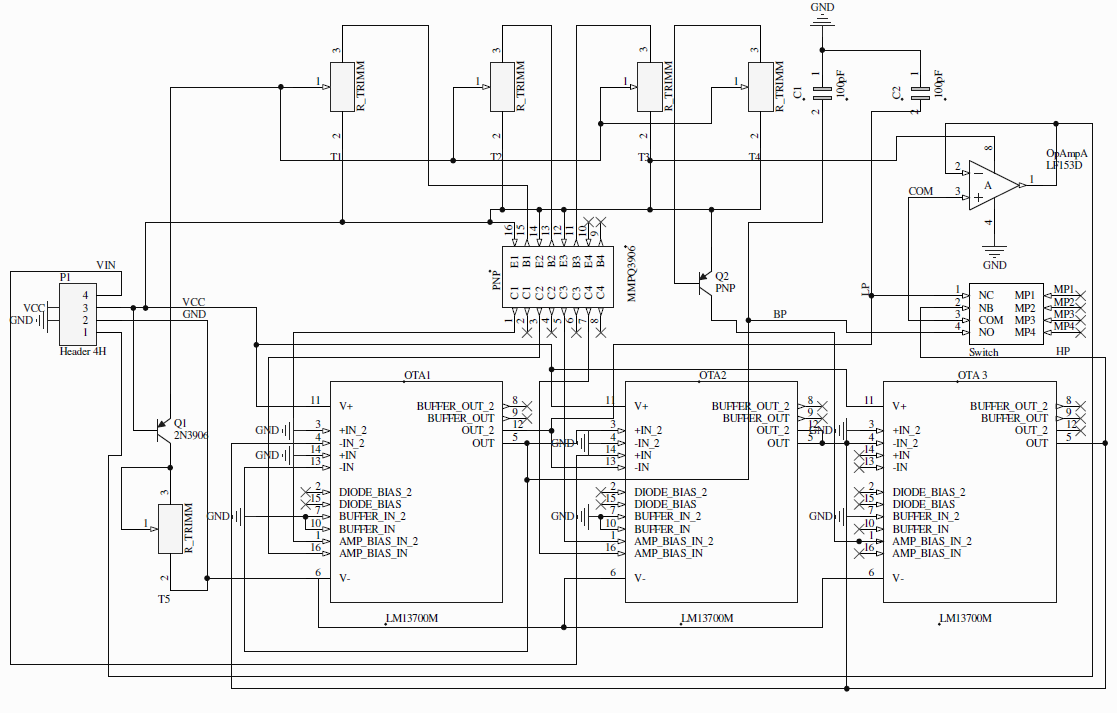
\includegraphics[scale=0.45]{v3schematics.png}
\caption{Schéma se zapojením IO s řízeným napájením}
\end{figure}
\begin{figure}[h]
\centering
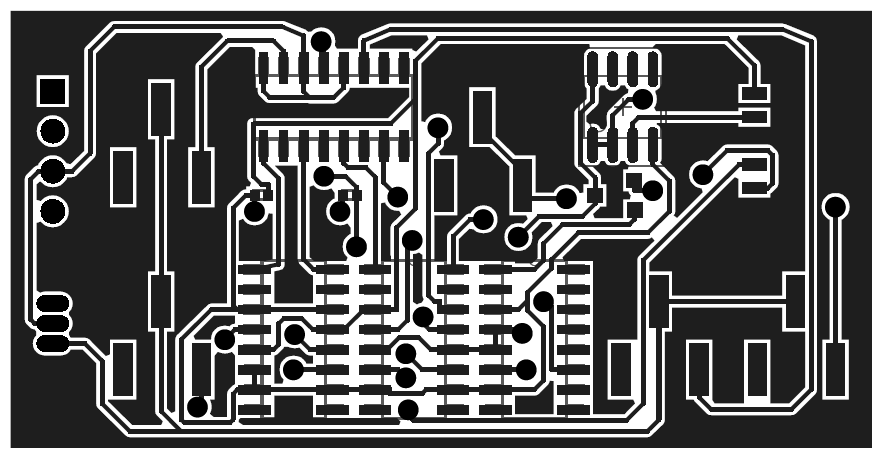
\includegraphics[scale=0.5]{v3top.png}
\caption{Horní strana DPS}
\end{figure}
\begin{figure}[h]
\centering
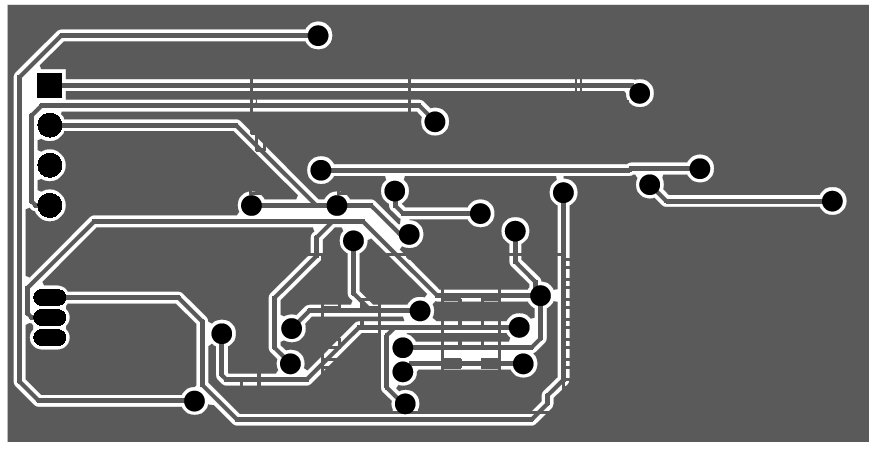
\includegraphics[scale=0.5]{v3bot.png}
\caption{Spodní strana DPS}
\end{figure}
\begin{figure}[h]
\centering
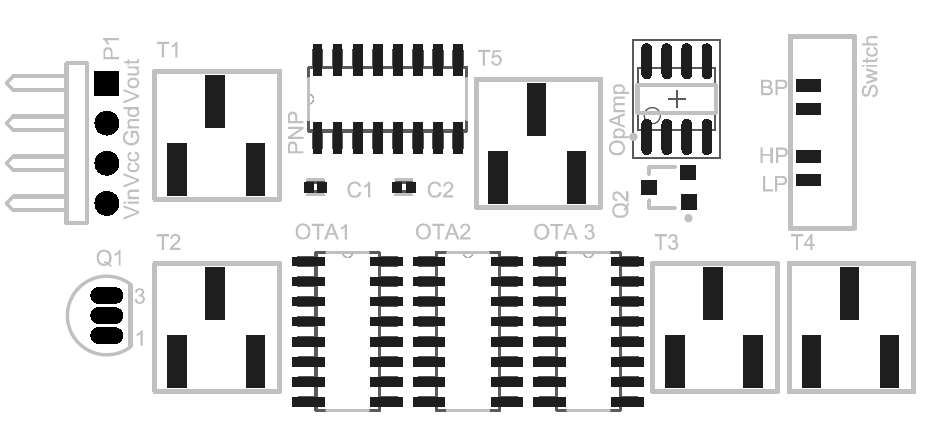
\includegraphics[scale=0.5]{v3assembly.png}
\caption{Rozmístění součástek}
\end{figure}
\begin{figure}[h]
\centering
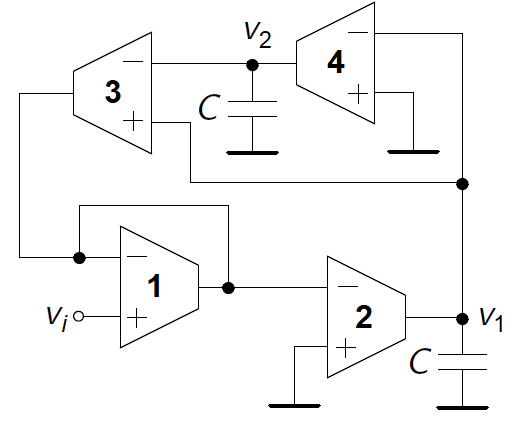
\includegraphics[scale=0.5]{v4.png}
\caption{Schéma zapojení OTA}
\end{figure}
\begin{figure}[h]
\centering
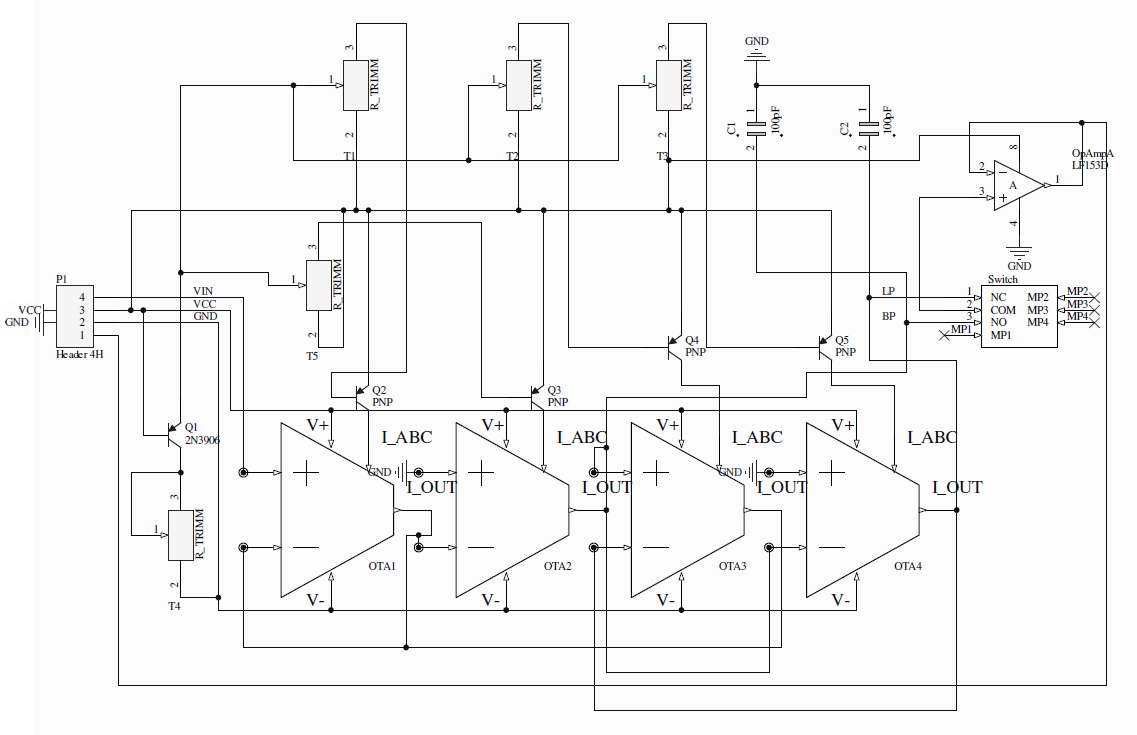
\includegraphics[scale=0.45]{schemev4.png}
\caption{Schéma s obvodovými prvky s řízeným napájením}
\end{figure}
\begin{figure}[h]
\centering
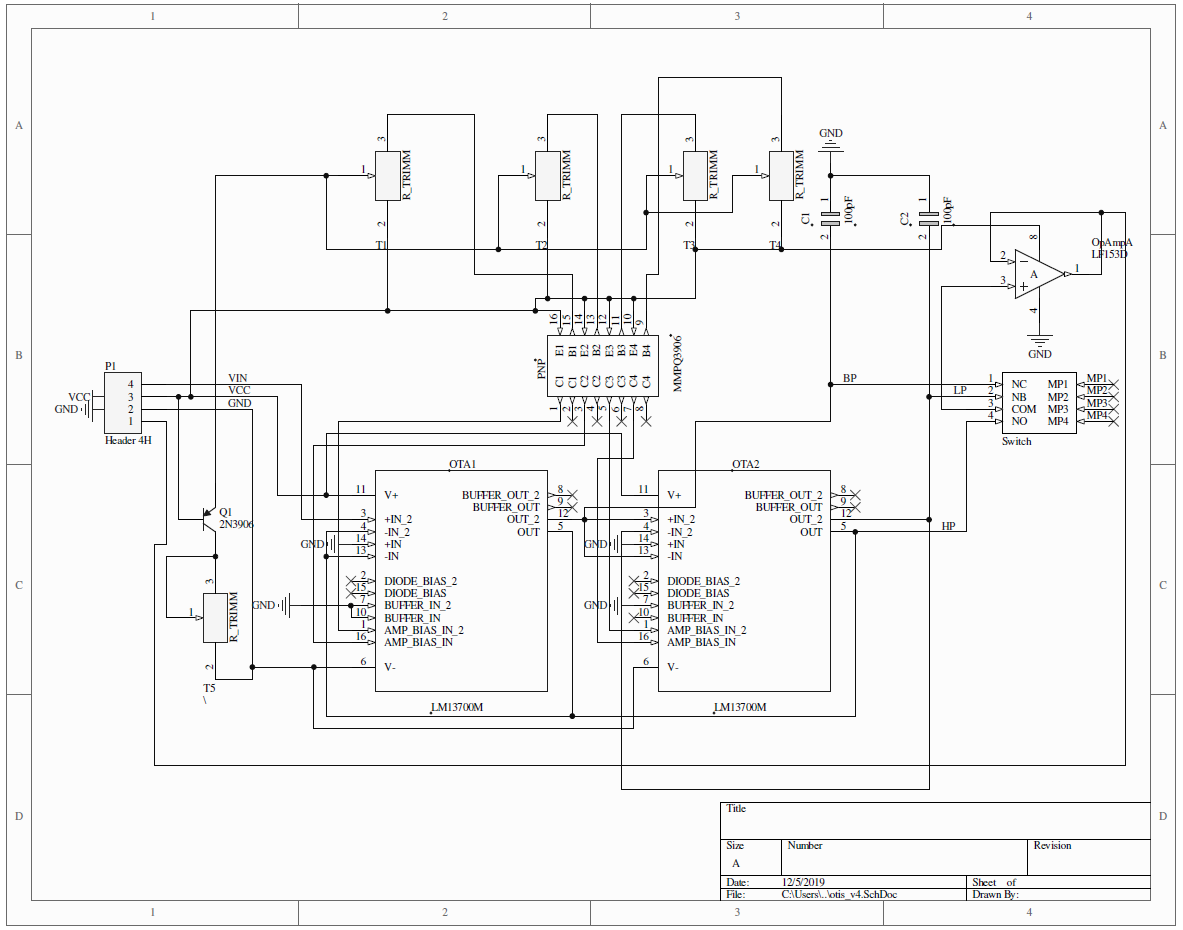
\includegraphics[scale=0.45]{v4schematics.png}
\caption{Schéma se zapojením IO s řízeným napájením}
\end{figure}
\begin{figure}[h]
\centering
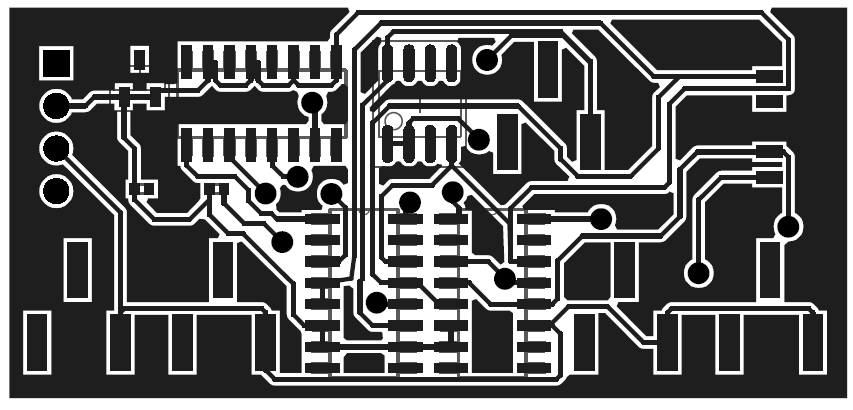
\includegraphics[scale=0.5]{v4top.png}
\caption{Horní strana DPS}
\end{figure}
\begin{figure}[h]
\centering
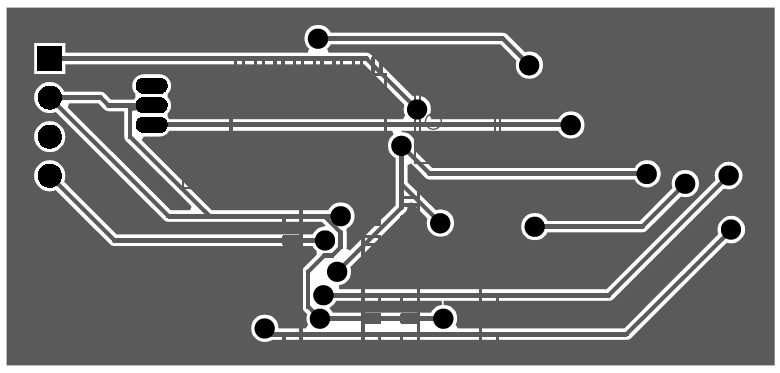
\includegraphics[scale=0.5]{v4bot.png}
\caption{Spodní strana DPS}
\end{figure}
\begin{figure}[h]
\centering
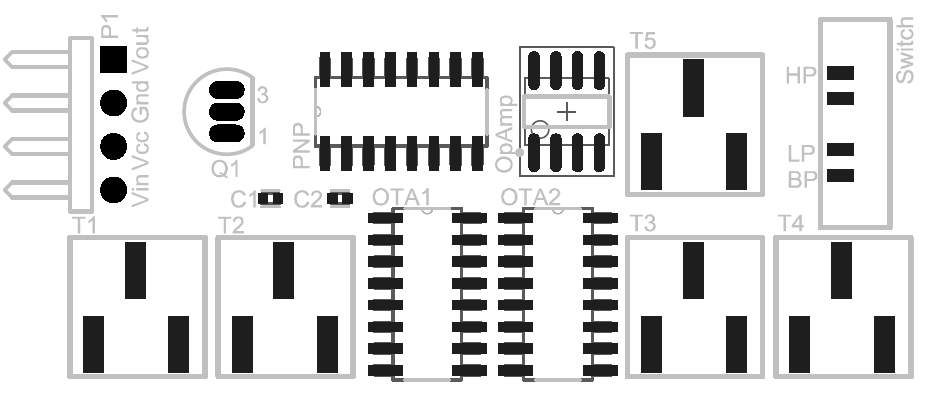
\includegraphics[scale=0.5]{v4assembly.png}
\caption{Rozmístění součástek}
\end{figure}